\section{Prompt Design}
\label{sec:method}
% We describe the iterative methodology of designing prompts with users' feedback, which will be listed in bullet point in this section. 

% Our prompt engineering for chatbots was based on (i) the objectives proposed by psychiatrists (see Section \ref{sec:objectives}), (ii) the process of ``trial and error'', and (iii) the feedback of psychiatrists. In this part, we will discuss the design process in detail.
% \KZ{I'm assuming in the trial and error stage, you will involve
% the human doctors and patients and get their feedback. But how is this process
% actually playing out? How is it different from the final evaluation which also
% consists of human and automatic evaluation. It's a little confusing.
% I think sec 4 - 7 need to be re-organized according to the two-stage
% methodology and redesign what to put into the final evaluation section.}
% In this part, we will discuss the design process in detail.
Based on the objectives obtained in Phase 1, we started prompt engineering, which is always iterative and full of ``trial and error''.

\subsection{Design Methodology}
When designing prompts for a chatbot, it is common practice to involve humans in conversing with the chatbot for each version of the prompt. However, common applications can involve general public as human judges, while in our practice, real users (i.e., doctors and patients) are necessary to be involved to meet the requirements of real-world applications. While human engagement is essential for prompt engineering, it can also make the iterative design process time-consuming and resource-intensive.

Inspired by \citet{deriu-etal-2020-spot}, we utilize a ``bot-to-bot'' method to generate dialogue history and collect user feedback based on it. 
% \KZ{One potential issue with bot-to-bot approach, is that the initial
% version of the doc bot and patient bot must be good enough to generate
% reasonable logs.} 
Instead of the conventional ``bot-to-human'' approach, we facilitate autonomous conversations between the doctor chatbot and the patient chatbot. By leveraging this autonomous interaction, we generate dialogue history that reflects potential user interactions. These generated chat logs are then presented to real psychiatrists, who provide valuable feedback and insights based on their expertise. 
This approach allows us to simulate user interactions without requiring direct human involvement, thereby reducing the time and resources needed for the iterative design process. Moreover, we can make informed improvements and refine the chatbot in subsequent iterations by incorporating the input of healthcare professionals.

\subsection{Doctor Chatbot}
\label{sec:doc_prompt}
As illustrated in  \figref{fig:doc_prompt_design}, we undergo three iterations to develop the prompt for the doctor chatbot, and the final version is presented below:
\begin{prompt}
    \ding{192} Please play the \uline{role} of an \uline{empathetic and kind} psychiatrist. 
    \ding{193} Your \uline{task} is to conduct a professional diagnosis conversation with me based on the DSM-5 criteria. 
    \ding{194} Your questions should \uline{cover at least the following aspects}: [\ldots]\protect\footnotemark. 
    % You are free to choose the order of questions, but you must collect complete information on all aspects in the end. 
    \ding{195} Please only ask \uline{one question at a time}.
    % , and each question should only cover one symptom.
    \ding{196} You need to ask \uline{in-depth questions}, such as the \Blue{duration}, \Blue{causes} and specific \Blue{manifestations}. 
    \ding{197} You need to use various \uline{empathetic strategies}, such as \Yellow{understanding}, \Yellow{support} and \Yellow{encouragement}. 
\end{prompt}
\footnotetext{The aspects include ``emotion'', ``sleep'', etc. We provide the full list in Appendix \ref{apd:prompts}.}

\begin{figure}[th]
	\centering
	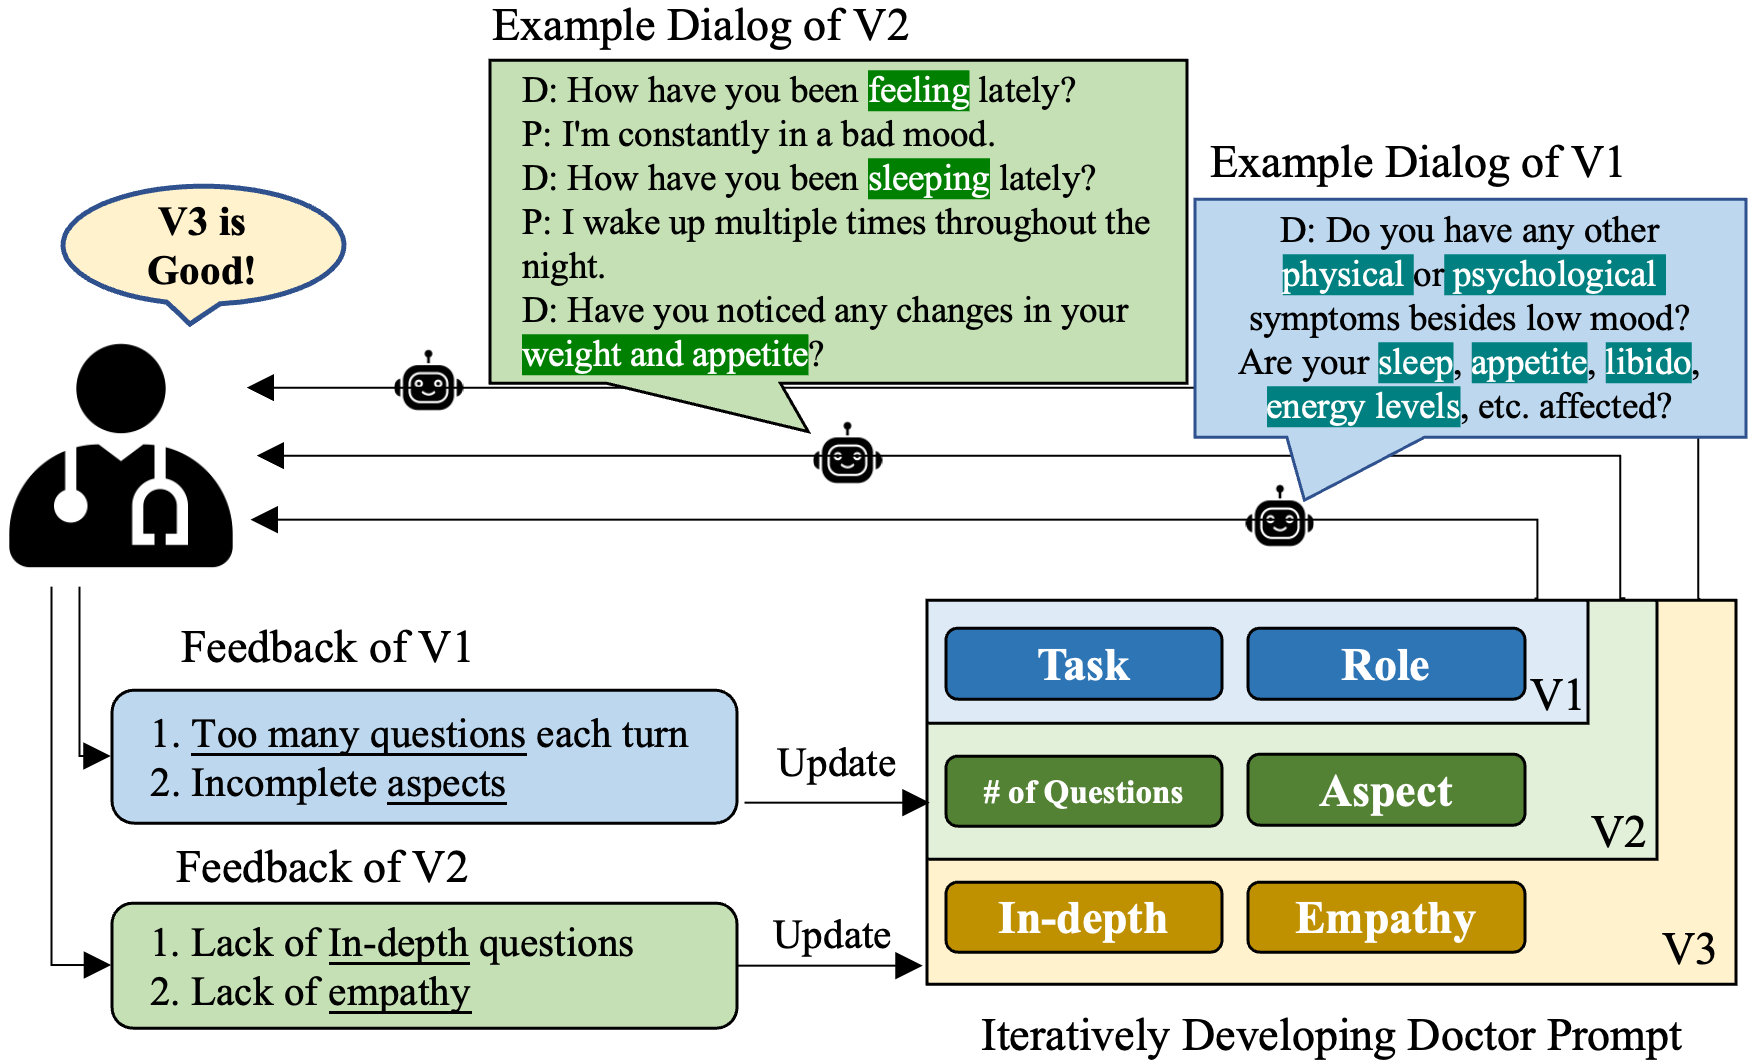
\includegraphics[width=\linewidth]{Figures/doctor_prompt_design.png}
	\caption{The iterative development process of the prompt of doctor chatbots. Psychiatrists will identify the limitations of the current version, and we will address these issues in the subsequent version.}
	\label{fig:doc_prompt_design}
\end{figure}
In this prompt, we provide a clear description of the task and establish the role to be simulated by the doctor chatbot. Then, we list the specific aspects that the doctor chatbot should cover during the questioning process. This serves as a guideline to ensure the \textit{comprehensiveness} objective. What's more, we include examples (highlighted in colored boxes) in the prompt to guide the doctor chatbot in asking \textit{in-depth} questions and demonstrating \textit{empathy}. These examples are crucial because, without them, the chatbot tends to ask superficial questions and  rely on generic phrases like ``thank you very much for your answer'' to show empathy. This arises from ChatGPT's limited comprehension of ``in-depth questioning'' and ``empathy'' in clinical contexts. Consequently, providing examples can be a promising approach to help ChatGPT grasp certain specialized skills within professional domains.

\subsection{Patient Chatbot}
\label{sec:pat_prompt}
After two iterations, we arrive at the final version of the prompt for the patient chatbot, which is presented below:
\begin{prompt}
    \ding{192} Please play the \uline{role} of a patient, who is currently chatting with a doctor. 
    \ding{193} \uline{You are experiencing the following symptoms}: [\texttt{Symptom List}]\protect\footnotemark 
     % \KZ{Instead of giving the full list of symptoms in the prompt, shouldn't we give a random subset of those symptoms?}
    \ding{194} Please talk to me based on the above symptom list. 
    \ding{195} You can only mention \uline{one symptom per round}. 
    \ding{196} You should \Blue{express} your symptoms in a \uline{vague and colloquial} way, and relate them to your \uline{life experiences}.
    \ding{197} You can have \Blue{emotional fluctuations} during the conversation. 
    \ding{198} You have a \Blue{resistance} towards doctors, and do not want to reveal some feelings easily.
\end{prompt}
\footnotetext{The symptom list is summarized by ChatGPT and revised by psychiatrists. See Appendix \ref{apd:symp_list} for details.}

In the first iteration, we describe the task (sentence \ding{192}\ding{193}), provide a symptom list (sentence \ding{194}) in the prompt, and add sentence \ding{195} to avoid listing all the symptoms in one turn. 
This prompt enables the chatbot to meet the basic requirement of providing \textit{honest} responses in most cases.
However, feedback from psychiatrists indicates that the chatbot lacks resemblance to real patients as it does not effectively convey \textit{emotions}, use colloquial \textit{expressions}, or demonstrate \textit{resistance} to seeking help. 

Therefore, we add sentence \ding{196}, \ding{197}, \ding{198} to address these issues in the second iteration.
However, we observe that the effect of adding these sentences is most prominent in the initial rounds of conversation, suggesting that the patient chatbot tends to forget some of the instructions given at the beginning. 
This behavior is reasonable considering ChatGPT's training objective to be a helpful, polite AI assistant that provides detailed responses. Consequently, there can be a potential mismatch between the desired behavior of the patient chatbot, including resistance and emotional fluctuations, and the training objective, making it more likely for these instructions to be forgotten.

To address this issue, we insert new reminders during the conversation. Inspired by the fact that the latter part of the prompt has the greatest impact on the responses generated by ChatGPT, our method is straightforward yet effective. Without users' awareness, we covertly append the following words at the end of the most recent sentence in the dialogue history.

\begin{prompt}
    (\Yellow{Attention:} colloquial language, life experience, low mood or mood swings, refuse or answer briefly due to resistance)
\end{prompt}

We aim to use simple phrases or words as reminders during the conversation to ensure that the sentences are not overly long. Moreover, these reminders are only temporarily attached to the most recent round, and will not persist in the dialogue history for subsequent rounds.
% With these reminders, the patient chatbot can maintain a colloquial language style consistently and exhibit resistance even in the latter part of the conversation, so we consider this version as the final one\footnote{The final version is in Table \ref{tab:patient_prompt} in Appendix \ref{apd:prompts}.}.

